\ifspanish

\question Consid\'{e}rese la observaci\'{o}n
			 $$ X = S + N  $$
con la se\~{n}al $S$ inmersa en un ruido $N$ independiente de ella, y siendo sus densidades de probabilidad 
		      $$p_S(s) =
			      \left\{\begin{array}{ll}
				  	\displaystyle
						  1, & 0<s<1 \\
						  0, & {\mbox{en otro caso}} 
 					 \end{array} 
				  \right. = \Pi (s - 1/2)
		      $$   
		      $$p_N(n) =
			      \left\{\begin{array}{ll}
				  	\displaystyle
						  1, & -1/2<n<1/2 \\
						  0, & {\mbox{en otro caso}} 
 					 \end{array} 
				  \right. = \Pi (n)
		      $$   
Establ\'{e}zcase el estimador de error cuadr\'{a}tico medio m\'{\i}nimo de $S$, $\hat{S}_\text{MMSE}$. Disc\'{u}tase el resultado.

\begin{solution}
   $\hat S_\text{MMSE} = \dfrac{1}{2} \left(X + \dfrac{1}{2}\right) \quad\quad (-1/2 < x <1/2) $       
   
   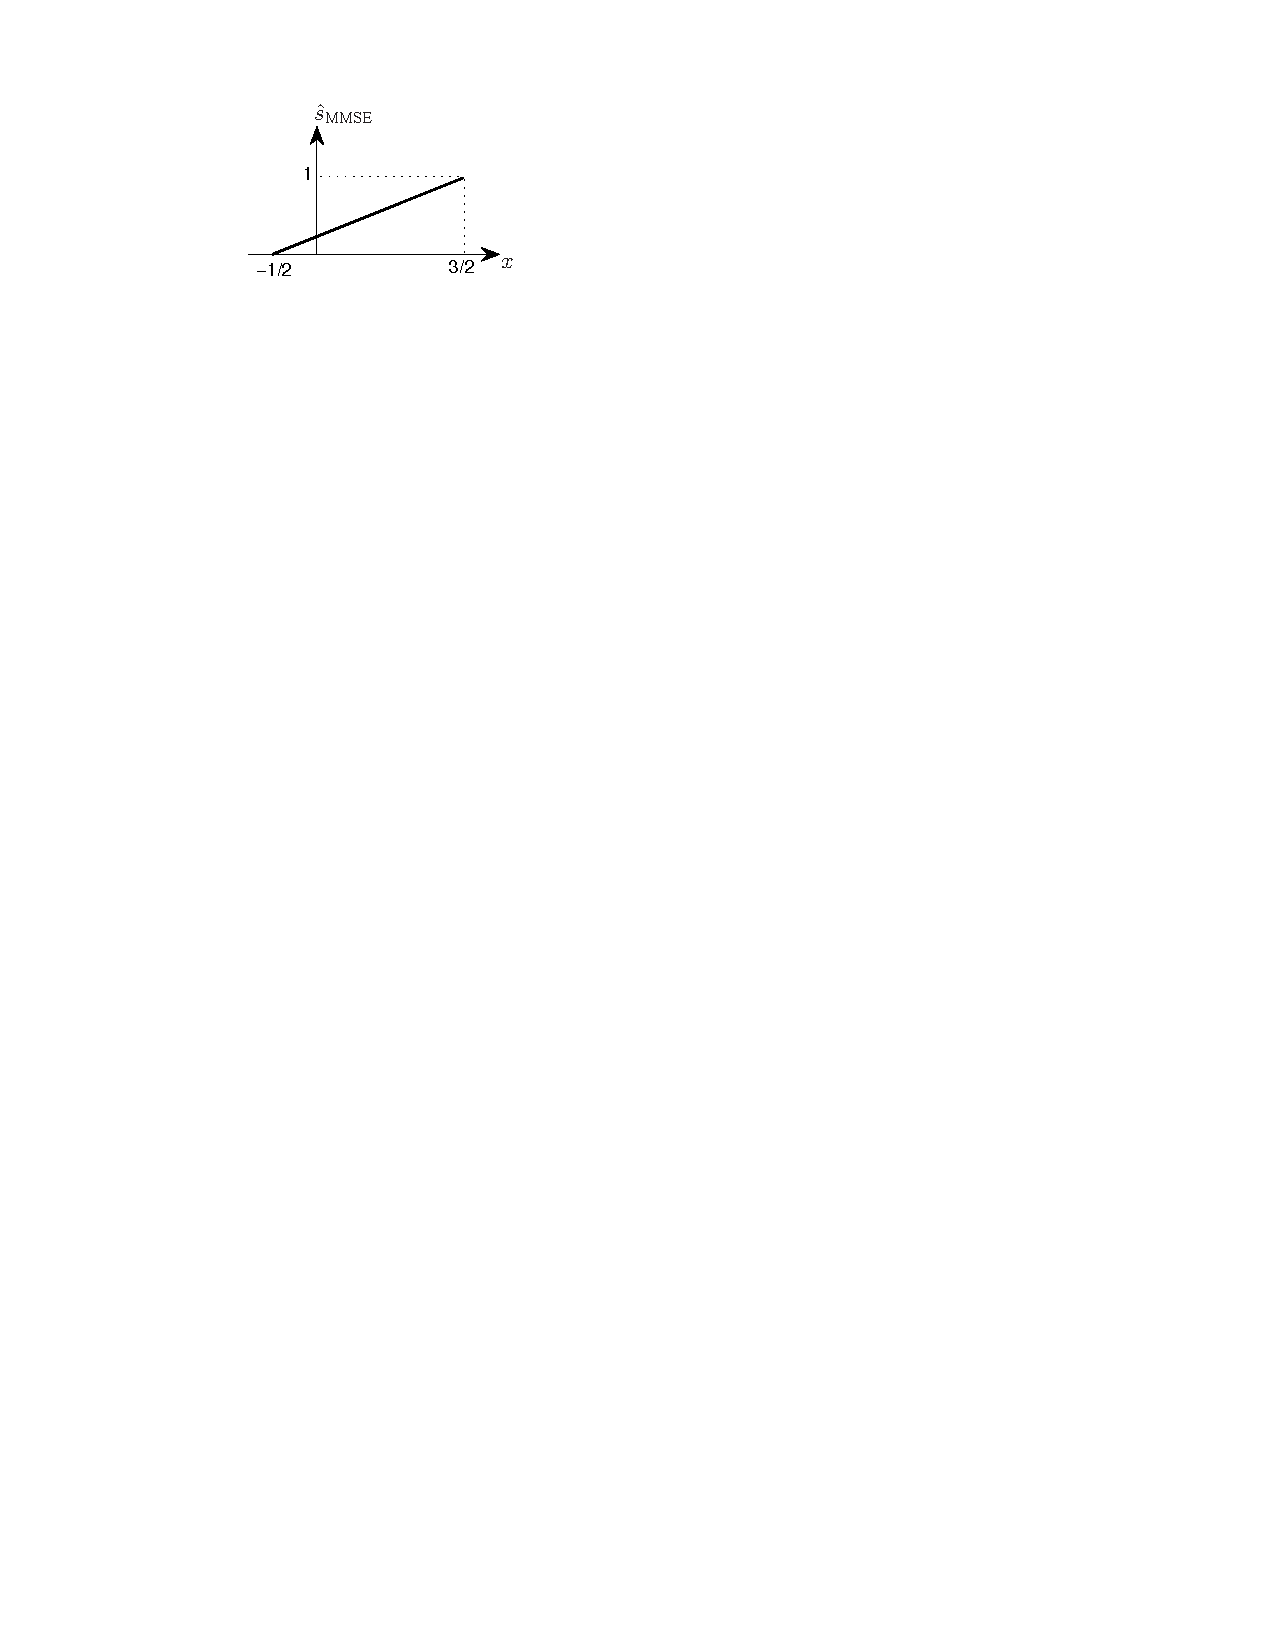
\includegraphics[width=8cm, trim=0 23cm 12cm 2cm]{Figuras/fig3E1}
   
   Las variaciones entre los casos extremos $(\hat{s}_\text{MMSE} (-1/2) = 0, \hat{s}_\text{MMSE} (3/2) = 1)$ se atribuyen linealmente al ruido
\end{solution}

\else

\question Consider an observation
					 $$ X = S + N  $$
					 where $S$ is  a signal contaminated by additive noise $N$, and where $S$ and $N$ are independent of each other, and with probability density functions given by:
				      $$p_S(s) =
					      \left\{\begin{array}{ll}
						  	\displaystyle
								  1, & 0<s<1 \\
	  							  0, & {\mbox{otherwise}} 
	 					 \end{array} 
						  \right. = \Pi (s - 1/2)
				      $$   
				      $$p_N(n) =
					      \left\{\begin{array}{ll}
						  	\displaystyle
								  1, & -1/2<n<1/2 \\
	  							  0, & {\mbox{otherwise}} 
	 					 \end{array} 
						  \right. = \Pi (n)
				      $$   
	 Find the minimum mean square error estimator of $S$, $\hat{S}_\text{MMSE}$. Discuss your result.

\begin{solution}
   $  \hat S_\text{MMSE} = \displaystyle\frac{1}{2} \left(X + \displaystyle\frac{1}{2}\right) \quad  \quad (-1/2 < x <1/2) $    
   
   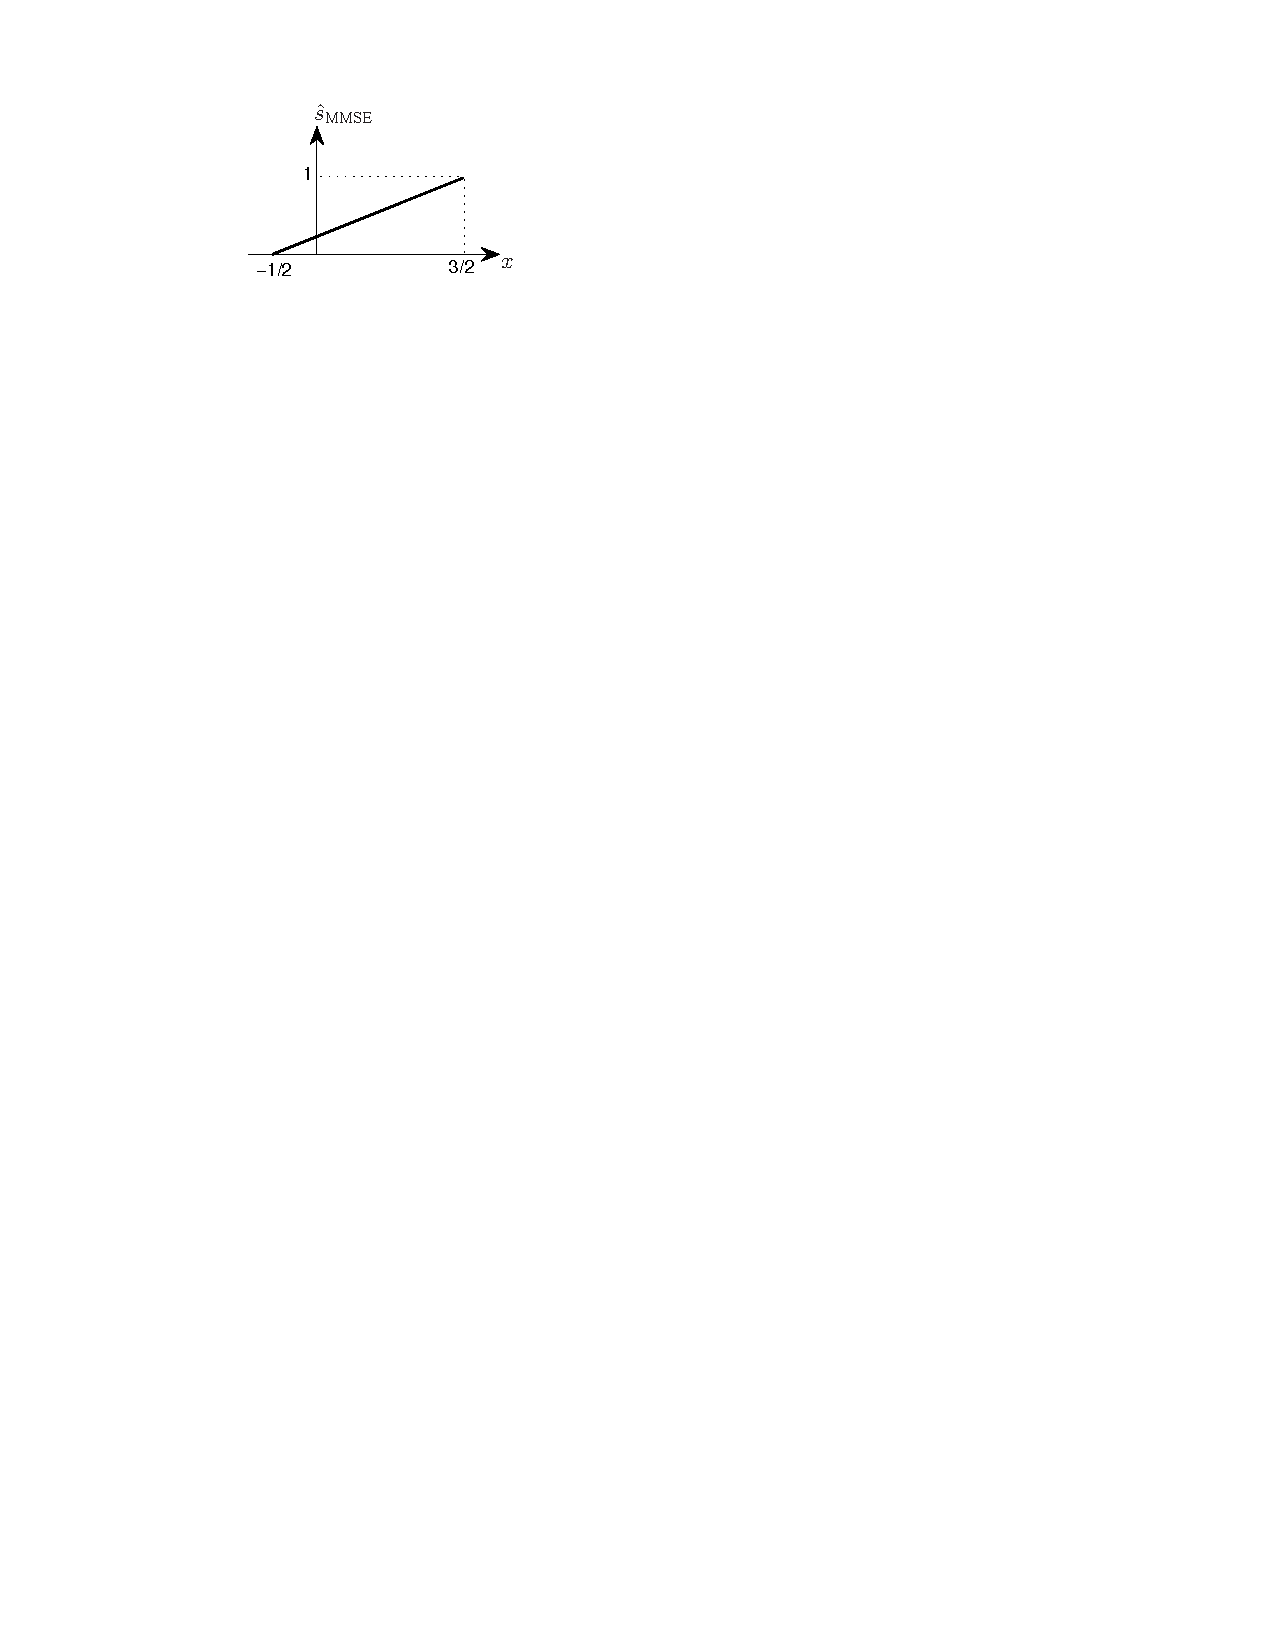
\includegraphics[width=8cm, trim=0 23cm 12cm 2cm]{Figuras/fig3E1}
   
   The linear change of the estimator between its minimum and maximum values $(\hat{s}_\text{MMSE} (-1/2) = 0, \hat{s}_\text{MMSE} (3/2) = 1)$ are due to the addition of uniform noise.
   \end{solution}

\fi